\documentclass[12pt]{report}
\usepackage[spanish, activeacute]{babel}
\usepackage[top=2.75cm,bottom=2.50cm,left=3.00cm,right=2.50cm]{geometry}
\usepackage[utf8]{inputenc}  
\usepackage{enumerate}
\usepackage{graphicx}



\begin{document}
	\setlength{\topmargin}{-0.5in}
	\pagestyle{empty}
	\begin{center}
		\textbf{
			\vspace{-0.7em}
			ESCUELA SUPERIOR POLITÉCNICA DEL LITORAL
		}
		\line(1,0){380}\\		
		\scriptsize{FACULTAD DE INGENIERÍA EN ELECTRICIDAD Y COMPUTACIÓN}
	\end{center}

	\begin{center}
		\vspace{2.5em}
		\Huge{\textbf{\\PROYECTO FINAL}}
	\end{center}	

	\begin{center}
		\Huge{\textbf{\\Recopilación de Trabajos II Término 2012	\vspace{1em}}}
	\end{center}
	\begin{center}
		\Huge{\textbf{\\Ana Arias	\vspace{1em}}}
		\\ acarias@espol.edu.ec
	\end{center}
	\begin{center}
		\Huge{\textbf{\\Lenguajes de Programación\vspace{1em}}}
	\end{center}	
	\begin{center}
		\Huge{\textbf{\\Ing. Javier Tibau	\vspace{1em}}}
		\\ jtibau@espol.edu.ec
		\\ jtibau@fiec.espol.edu.ec
	\end{center}	



\chapter*{Agradecimientos}
\addcontentsline{toc}{chapter}{Agradecimientos} 
\markboth{AGRADECIMIENTOS}{AGRADECIMIENTOS} % encabezado 
 
Quiero agradecer a mis compañeros de grupo y compañeros del aula, ya que entre todos compartimos conocimientos y buenas experiencias.
También quiero agradecer a mi profesor de Lenguajes de Programación Ing. Javier Tibau por darnos todos los retos de este semestre.

\chapter*{Resumen} 
\addcontentsline{toc}{chapter}{Resumen} 
\markboth{RESUMEN}{RESUMEN} % encabezado

Este documento contiene las descripciones y experiencias de los proyectos realizados en la materia Lenguajes de Programación dirigida por el Ing. Javier Tibau.

\tableofcontents


%---------------------------------------------------------------------------------------------------------------------------------
%--------------------------------------------------------------GITHUB!------------------------------------------------------
%---------------------------------------------------------------------------------------------------------------------------------
\chapter{Herramienta GitHub\label{capitulouno}}

	\begin{center}
		\begingroup
			
\includegraphics[width=0.27\textwidth]{imagenes_usuario/git.png}
		\endgroup
	\end{center}


	\begingroup
		\large{
			\textbf{
			           \newline
			           \newline
				Experiencias y Anécdotas: GitHub
				\newline
				\newline
			}
		}
	\endgroup
Mi experiencia con GitHub ha sido buena, esta herramienta en verdad mejoró la comunicación en los trabajos con mi grupo; lo que más me agradó es que podemos estar actualizados con respecto a las modificaciones en los archivos que nos tocó hacer de forma grupal, y por lo tanto se evita el compartir documentos frecuentemente a través de otra herramienta y la creación de un sinfín de documentos que contienen en realidad lo mismo.
\newline
\newline	
Considero Github como una red social, ya que podemos estar conectados con nuestros compañeros y compartir información, y además de ser social, es seria ya que a partir de esta herramienta se pueden encontrar trabajos muy interesantes de distintas personas, dicho material puede ser muy útil.
\newline
\newline	
Con respecto a su uso, lo considero sencillo y mecánico; al principio es un poco difícil aprender cómo se utiliza pero después se vuelve costumbre ya que los procedimientos para subir archivos, para crear repositorios, para modificarlos es en realidad muy mecánico.
\newline
Esta herramienta es una buena opción para dar a conocer nuestros trabajos en internet, y seguramente la seguiré utilizando en el futuro.
\newline
\newline
Mi experiencia con Github a lo largo del semestre pasó de ser mala, a regular y finalmente a muy buena. Esto tiene mucho que ver por toda la practica que tuvimos que tener con esta herramienta, ya que la utilizamos en todos los proyectos.
El uso de la herramienta Github se facilitó mucho cuando empecé a utilizar su interfaz.
\newline
	\begin{center}
		\begingroup
			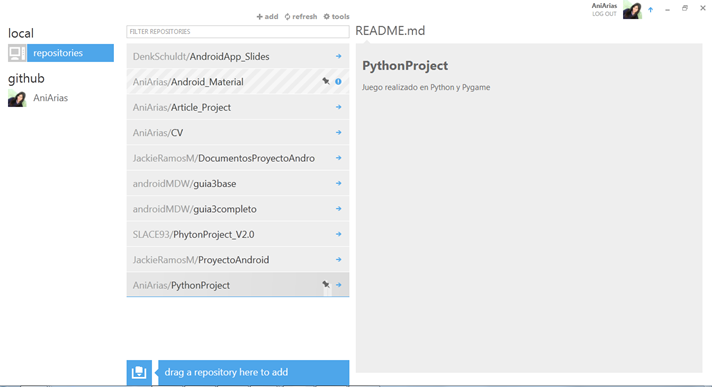
\includegraphics[width=0.8\textwidth]{imagenes_usuario/git2.png}
\newline
\newline
		\endgroup
	\end{center}

	\begin{center}
		\begingroup
			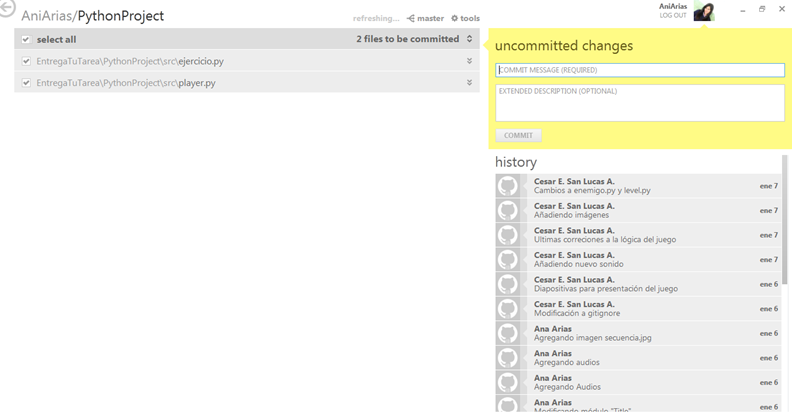
\includegraphics[width=0.8\textwidth]{imagenes_usuario/git3.png}
\newline
\newline
		\endgroup
	\end{center}

La interfaz de Github permite realizar commits de manera mucho mas rápida y mas detallada; me pareció mu interesante la rapidez con que se actualizaban los proyectos cada vez que se modificaba algo.
Recomendaría utilizar la interfaz de GitHub para las personas que recién empiecen a utilizar esta herramienta.
\newline
\newline
Seguiré utilizandola para futuros proyectos y en mi vida profesional.

 \ref{capitulouno}


%---------------------------------------------------------------------------------------------------------------------------------
%--------------------------------------------------------------LATEX------------------------------------------------------
%---------------------------------------------------------------------------------------------------------------------------------


\chapter{Herramienta LateX\label{capitulouno}}

	\begin{center}
		\begingroup
			
\includegraphics[width=0.27\textwidth]{imagenes_usuario/latex.jpg}
		\endgroup
	\end{center}


	\begingroup
		\large{
			\textbf{
				Experiencias y Anécdotas: LaTeX
				\newline
				\newline
			}
		}
	\endgroup

Latex es una buena opción al momento de la creación de documentos de distinto tipo, una herramienta que nos saca de la rutina de los mismos editores de texto que utilizamos a diario; y sin embargo Latex ofrece las mismas características que dichos editores.
\newline	
\newline	
Latex  a pesar de aparentar dificultad, es una herramienta sencilla de utilizar, solo es cuestión de conocer los comandos que permiten editar el formato de nuestro documento.
Otra ventaja de Latex es que existen plantillas para realizar distintos tipos de documentos, estas plantillas facilitan la edición del formato de un texto que quizás no sepamos cómo debería estar formado.
\newline	
\newline	
Como conclusión, el uso de esta herramienta me pareció entretenida y útil, además, fue un reto ya que como programadores debemos ser capaces de adaptarnos a cualquier herramienta.
\newline
\newline		
Existen muchos tutoriales de cómo utilizar Latex, los cuales fueron de mucha ayuda al momento de generar el primer documento que fue el CV, ya que al ser una herramienta nueva, tuve que introducirme al uso de ésta y cuáles son las mejores cualidades que ofrece; para este artículo tengo más experiencia y me costó menos tiempo hacerlo y se me hizo mucho más entretenido.
\newline
Nuestra primera tarea en Latex fue el Curriculum Vitae, al principio el uso de latex, al ser algo nuevo para mi, fue un poco tedioso sin embargo en internet se encuentran muchos tutoriales para crear simpaticos documentos de distintos tipos; se encuentran un sin fin de plantillas que ayudan a empezar a aprender a programar y decorar mucho mejor los documentos que queramos realizar.
Con el tiempo cada vez se hizo mas fácil su uso.
\newline
Lo que me causó mas problema con esta herramienta eran los paquetes que se tenian que instalar para hacer funcionar algunas plantillas, ya que la instalación de estos paquetes a veces era muy rápida y otras veces muy lenta.

La realizacion de mi Curriculum Vitae fue muy útil, ya que éste me ha servido ya en múltiples ocasiones.

El uso de Latex no es cosa del otro mundo, sin embargo existen muchos comandos que sirven para dar formato a nuestros documentos, debemos utilizarlos correctamente ya que si nos olvidamos de cerrar algún bloque de texto o una sentencia, nuestro programa no se compliará de manera exitosa.
\newline
\newline
\newline
\newline
\newline
\newline
\newline
\newline
\newline
\newline
\newline
\newline
\newline
\newline
\newline
\newline
\newline
\newline
\newline
\newline
\newline
\newline
\newline
\newline
\newline
\newline
\newline
\newline

 \ref{capitulouno}


%---------------------------------------------------------------------------------------------------------------------------------
%--------------------------------------------------------------COMIC IT!------------------------------------------------------
%---------------------------------------------------------------------------------------------------------------------------------


\chapter{Proyecto Android \label{capitulodos}}
\begin{center}
		\Huge{\textbf{\\Comic It!	\vspace{1em}}}
\end{center}	


	\begingroup
		\large{
			\textbf{
				Objetivo General
				\newline
				\newline
			}
		}
	\endgroup
	Definir y dar a conocer las funcionalidades y los requerimientos que tendrá el proyecto para la materia Lenguajes de Programación de la Escuela Superior Politécnica del Litoral. 
\newline
\newline
Constrastar y relatar las experiencias vividas con GitHub y LaTeX.
	\vspace{4em}
	\newline
	\begingroup
		\large{
			\textbf{
				Objetivos Específicos
				\newline
			}
		}
	\endgroup
		\begin{enumerate}[(a)]%for small alpha-characters within brackets.
		\item Conocer las funcionalidades de la nueva aplicación para Android: Comic It!.
		\item Describir cada una de las funcionalidades que tendrá la aplicación.
		\item Especificar quiénes serán los usuarios finales de la aplicación.
		\item Presentar ciertas características que tendrá la aplicación final.
		\item Exponer experiencias con la instalación/utilización de GitHub y LaTex.
		\item Relatar anécdotas con la instalación/utilización de GitHub y LaTex.
		\end{enumerate}
	
	
\newpage
	\begingroup
		\large{
			\textbf{
				Descripción
				\newline
				\newline
			}
		}
	\endgroup

	%
	%Descripcion
	%
``Comic It!'' es una nueva aplicación para disposivos móviles que utilizan como sistema operativo Android. El nombre representa completamente a este nuevo software, puesto que será diseñado para crear historietas.
\newline
\newline
``Comic It!'' tendrá como usuarios a personas que les gusta tomar fotos y conservar recuerdos de los momentos divertidos que viven diariamente.
\newline
\newline
Con plantillas para colocar sus fotos, burbujas de diálogo e imágenes predeterminadas, el usuario quedará satisfecho cuando obtenga su obra final en su dispositivo.
\newline
\newline
Esta historieta relatará de una manera divertida, humorística y muy colorida exactamente lo que el usuario ha vivido o haya querido inventar para su uso personal.
	\newline
	\newline
	\newline
	\begingroup
		\large{
			\textbf{
				Funcionalidades
				\newline
				\newline
			}
		}
	\endgroup
	%
\newline
Comic It! cuenta con una variedad de funcionalidades que el usuario puede usar de manera rápida y dinámica utilizando 				fotos tomadas directamente de la CÁMARA o de la GALERÍA FOTOGRÁFICA .
\newline
\newline
El usuario tendrá la opción de crear un collage tipo caricatura  con fotografías de la galería de fotos del celular en una plantilla escogida de una LISTA DE PLANTILLAS proporcionadas por la aplicación.
\newline
\newline
Comic It! cuenta con una LISTA DE ÍCONOS básicos y personalizados que permitirán al usuario crear imágenes más reales y divertidas.	
\newline
\newline	
Además de íconos, el usuario tendrá una LISTA DE TEXTOS divertidos para darle mas creatividad a las escenas que esté creando.
\newline
\newline
Proporciona una lista con varios formatos de BURBUJAS DE DIALOGO, de las cuales el usuario puede escoger las que más se ajuste a su necesidad. El usuario podrá EDITAR EL TEXTO dentro de la burbuja de dialogo que haya escogido, convirtiendo a los miembros de 		la fotografía en auténticos personajes.
\newline
\newline
Al terminar de crear caricaturas, se podrán guardar en la galería fotográfica en distintos FORMATOS.

\newpage
	\begingroup
		\large{
			\textbf{
				Ilustración	
				\newline
				\newline
			}
		}
	\endgroup
Este es un pequeño vistazo a como se espera que sea la aplicación, resaltando sus partes más importantes:
	\newline

	\begin{center}
		\begingroup
			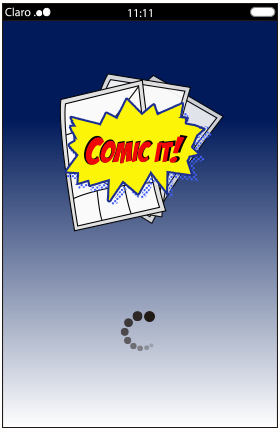
\includegraphics[width=0.19\textwidth]{imagenes_usuario/demo1.jpg}
		\endgroup
		\begingroup
			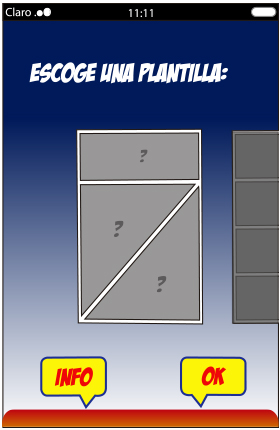
\includegraphics[width=0.19\textwidth]{imagenes_usuario/demo2.jpg}
		\endgroup
		\begingroup
			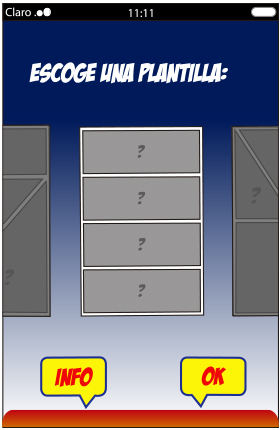
\includegraphics[width=0.19\textwidth]{imagenes_usuario/demo3.jpg}
		\endgroup
		\begingroup
			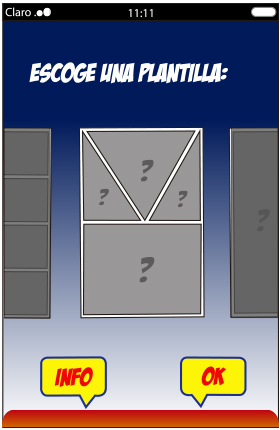
\includegraphics[width=0.19\textwidth]{imagenes_usuario/demo4.jpg}
		\endgroup
		\begingroup
			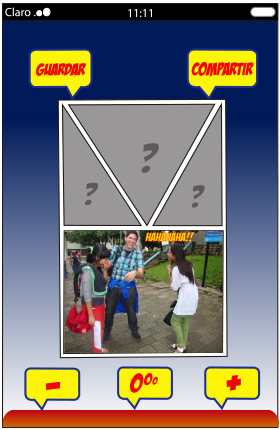
\includegraphics[width=0.19\textwidth]{imagenes_usuario/demo5.jpg}
		\endgroup
	\end{center}

\begingroup
			\vspace{3mm}
		\endgroup
Se observa la imagen inicial de la aplicación, seguido de las pantallas de selección de plantillas. Luego, puede verse un bosquejo de la aplicación en su parte más importante: La edición de la historieta.
 \newline
 \newline
En la parte superior, se tienen los botones 'Guardar' y 'Compartir'. Guardar, como su nombre lo indica, permitiría guardar la aplicación en la librería de imágenes del smartphone. 'Compartir' permitiría mostrar la historieta finalizada en las redes sociales, Twitter y Facebook.
 \newline
 \newline
En la parte inferior se observan los botones '-', '+'  y el botón de selección de burbujas. Los dos primeros botones servirían para redimensionar las burbujas o íconos en pantalla.

\newpage
\begin{center}	
	\vspace{1em}
		\Huge{\textbf{\\Manual de Usuario	\vspace{1em}}}
	\end{center}	


\begingroup
		\large{
			\textbf{
				Cargando la Cámara...
				\newline
				\newline
			}
		}
	\endgroup
Espere mientras la aplicación ComicIt! es cargada completamente.


	\begin{center}
		\begingroup
			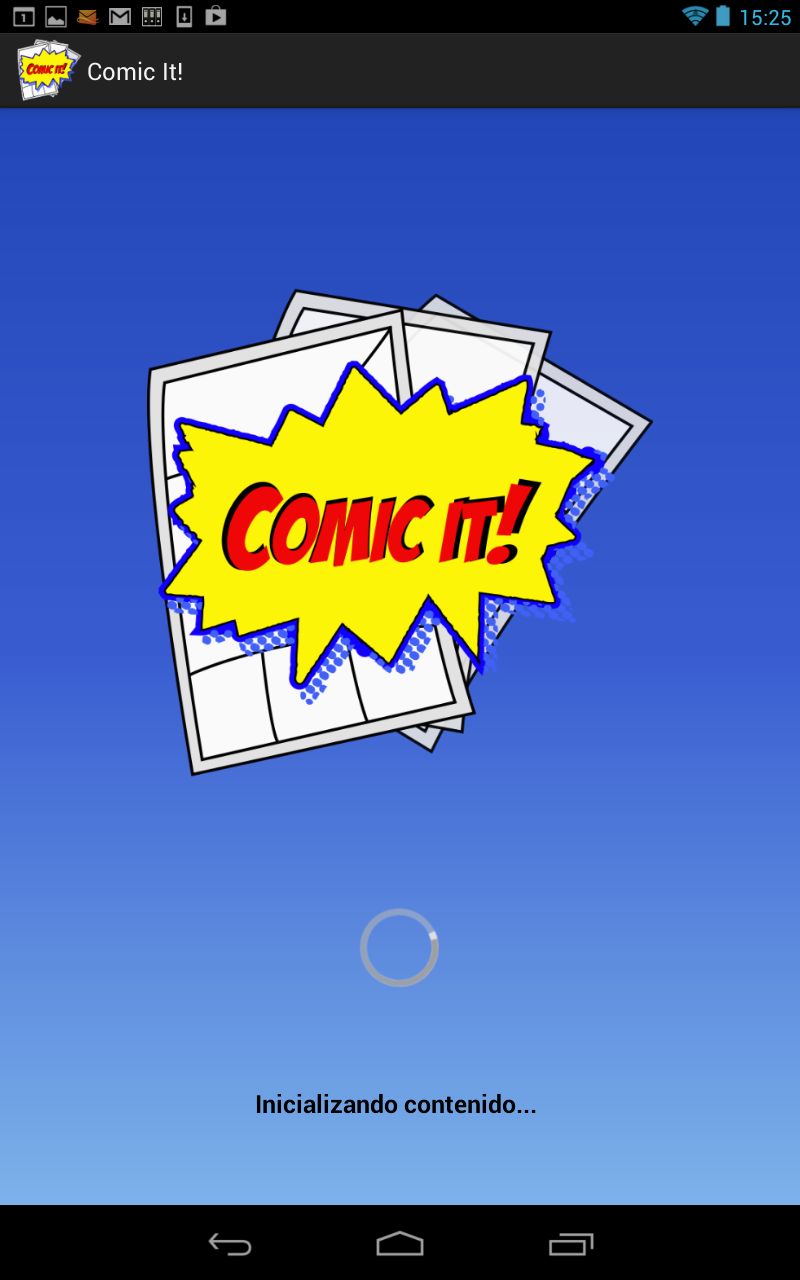
\includegraphics[width=0.27\textwidth]{imagenes_usuario/cargar.png}
		\endgroup
	\end{center}


\begingroup
		\large{
			\textbf{
				Escogiendo Plantilla...
				\newline
				\newline
			}
		}
	\endgroup
Al abrir la aplicación se encontrarán las opciones de plantillas, de las cuales el usuario puede escoger la que desee según el tipo de caricatura que desee crear; estas plantillas contienen la opción de colocar 5 imágenes, colocadas en distintas posiciones según el diseño de la plantilla.
				\newline
				\newline
	\begin{center}
		\begingroup
			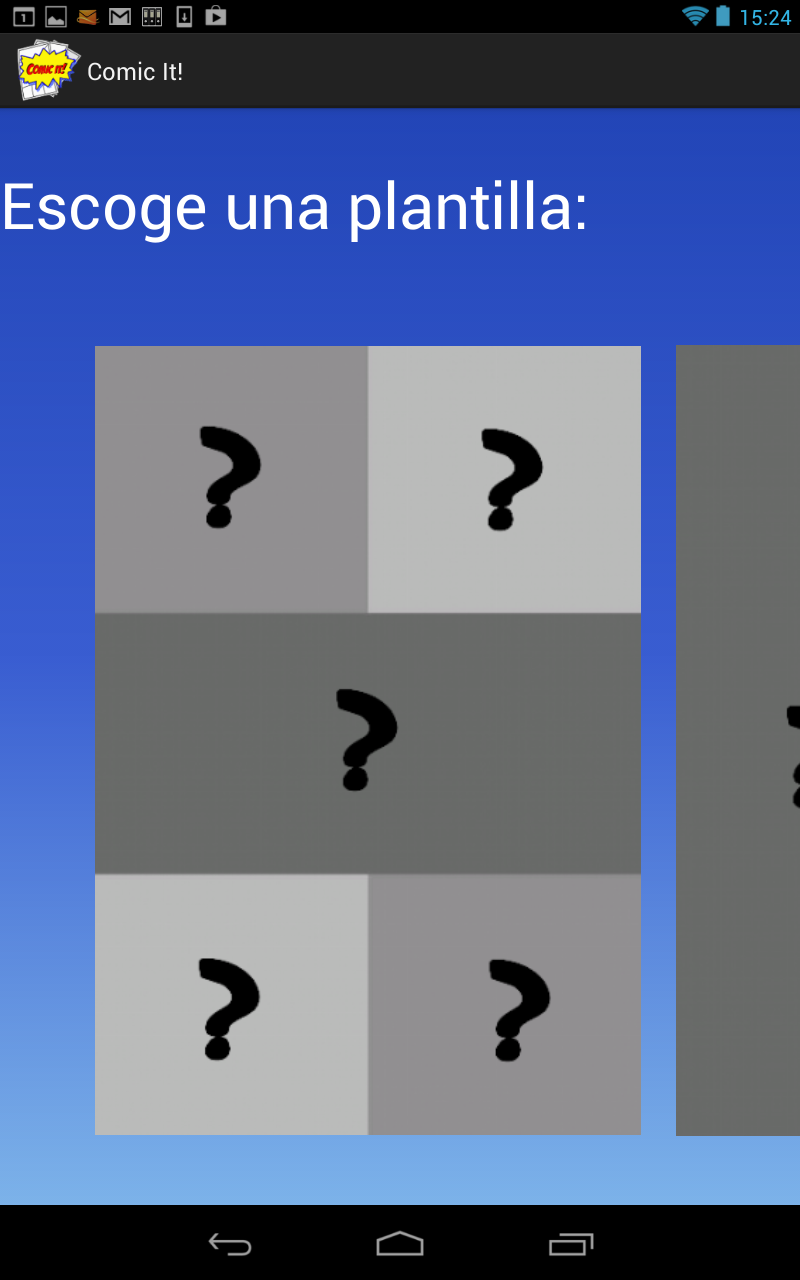
\includegraphics[width=0.24\textwidth]{imagenes_usuario/plantillas.png}
		\endgroup
	\end{center}


\begingroup
		\large{
			\textbf{
				Llenando Plantilla con fotos...
				\newline
				\newline
			}
		}
	\endgroup
Al darle un click a la plantilla que se desea escoger se abrirá una ventana en la cual la plantilla escogida saldrá en toda la pantalla. El usuario podrá empezar a crear su caricatura!
Para poder colocar fotos en los recuadros de la plantilla, el usuario tendrá que darle click al recuadro que desea rellenar con fotos tomadas ya sea desde la cámara o la galería de fotos del celular
\newline
\newline
	\begin{center}
		\begingroup
			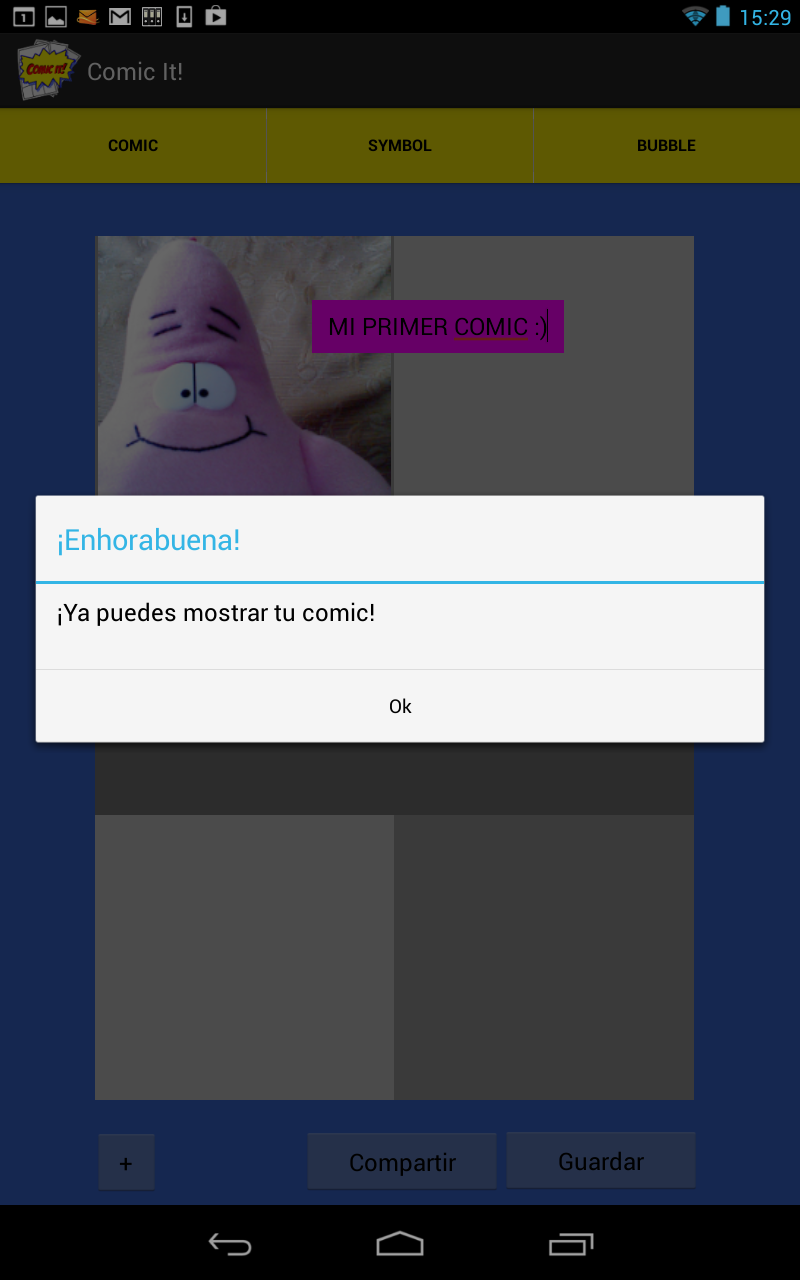
\includegraphics[width=0.27\textwidth]{imagenes_usuario/camara.png}

		\endgroup
	\end{center}


\begingroup
		\large{
			\textbf{
				Usando la Cámara...
				\newline
				\newline
			}
		}
	\endgroup
Si se escoge la opción cámara, automáticamente aparecerá la cámara del celular, de la cual se tomará la foto deseada.
\newline
\newline
\newline
	\begin{center}
		\begingroup
			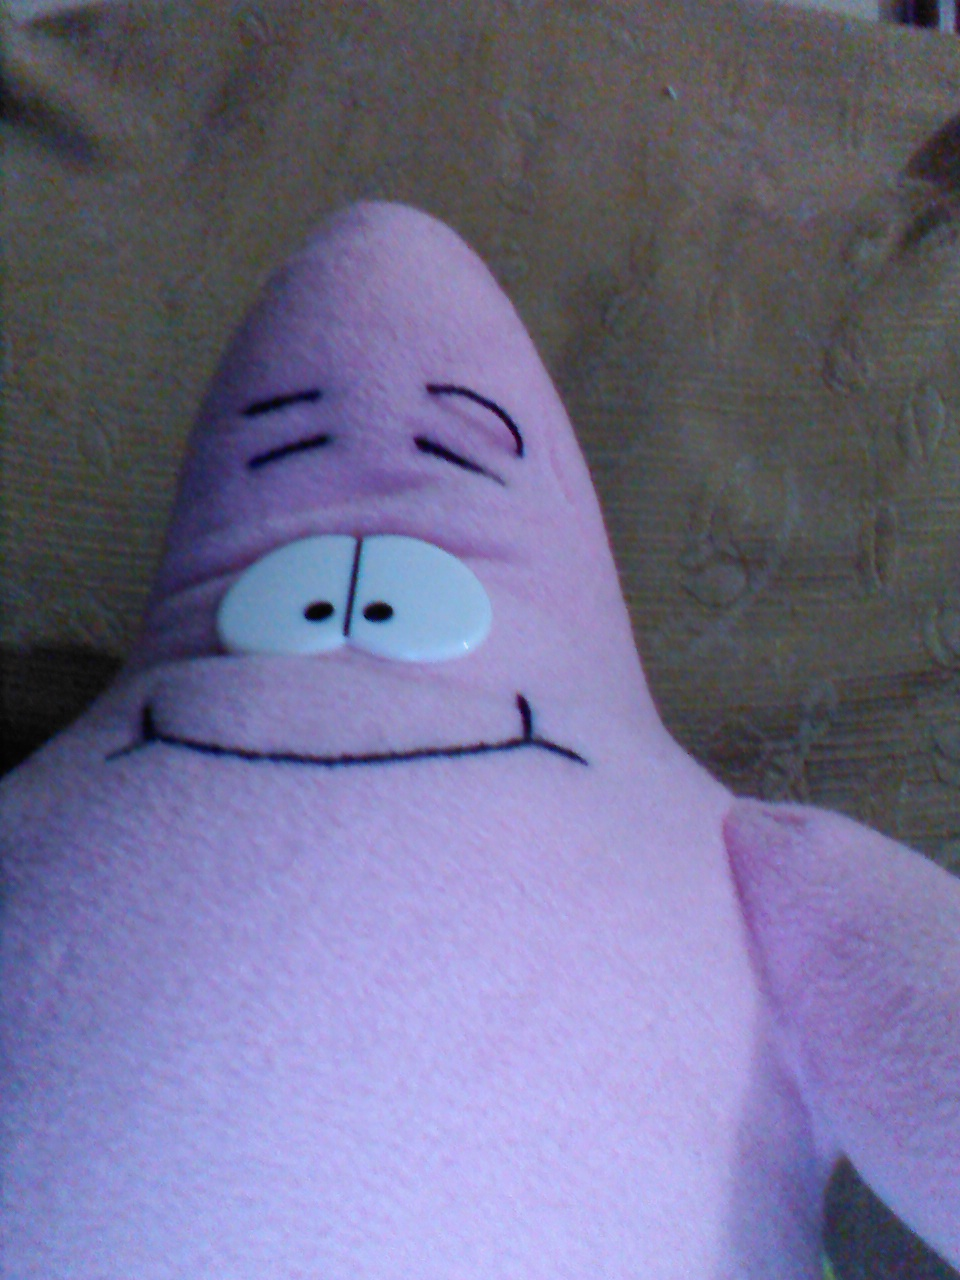
\includegraphics[width=0.27\textwidth]{imagenes_usuario/foto.jpg}
		\endgroup
	\end{center}



\begingroup
		\large{
			\textbf{
				Accediendo a la galería...
				\newline
				\newline
			}
		}
	\endgroup
Si por el contrario se escoge la galería de fotos, se abrirá automáticamente la galería fotográfica del celular, en la que se deberá buscar la foto deseada y escogerla.
\newline
\newline
	\begin{center}
		\begingroup
			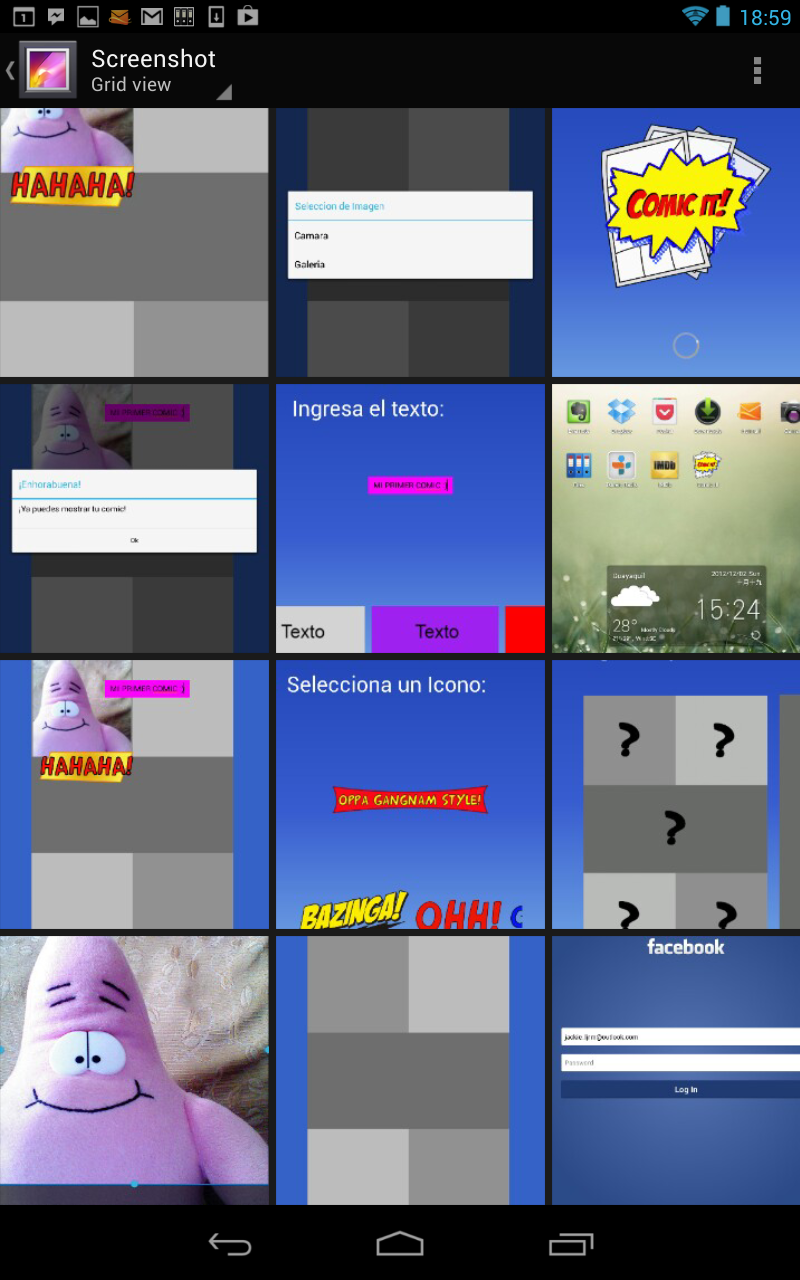
\includegraphics[width=0.27\textwidth]{imagenes_usuario/galeria.png}
		\endgroup
	\end{center}


\begingroup
		\large{
			\textbf{
				Recortando foto...
				\newline
				\newline
			}
		}
	\endgroup
Una vez obtenida la foto deseada, se creará automáticamente la opción para recortar dicha foto, y así determinar el rango de imagen que se desea de la foto tomada.
\newline
\newline
\newline
	\begin{center}
		\begingroup
			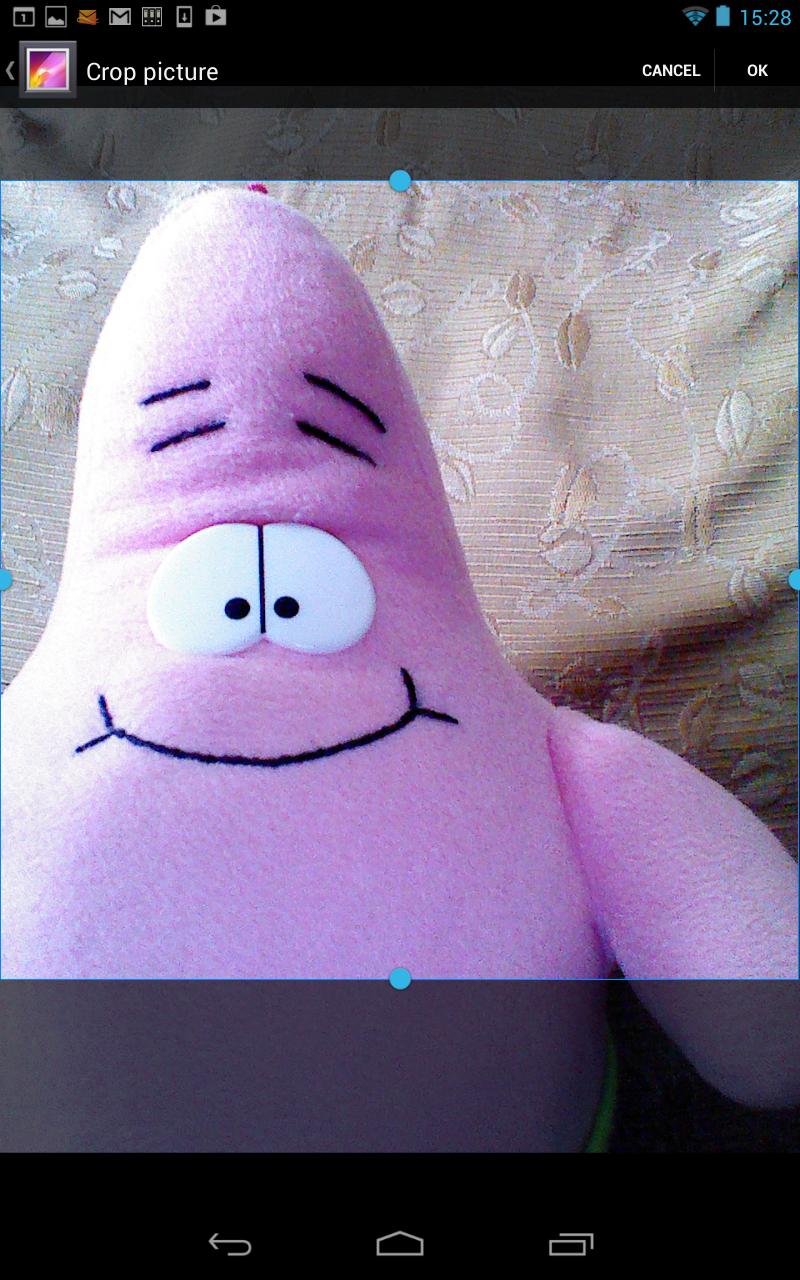
\includegraphics[width=0.27\textwidth]{imagenes_usuario/crop.png}
		\endgroup
	\end{center}


Luego de recortar la imagen y aceptar, la imagen obtenida y recortada se colocará en el recuadro que escogimos. Se debe repetir el proceso para los demás recuadros en la plantilla.
\newline
	\begin{center}
		\begingroup
			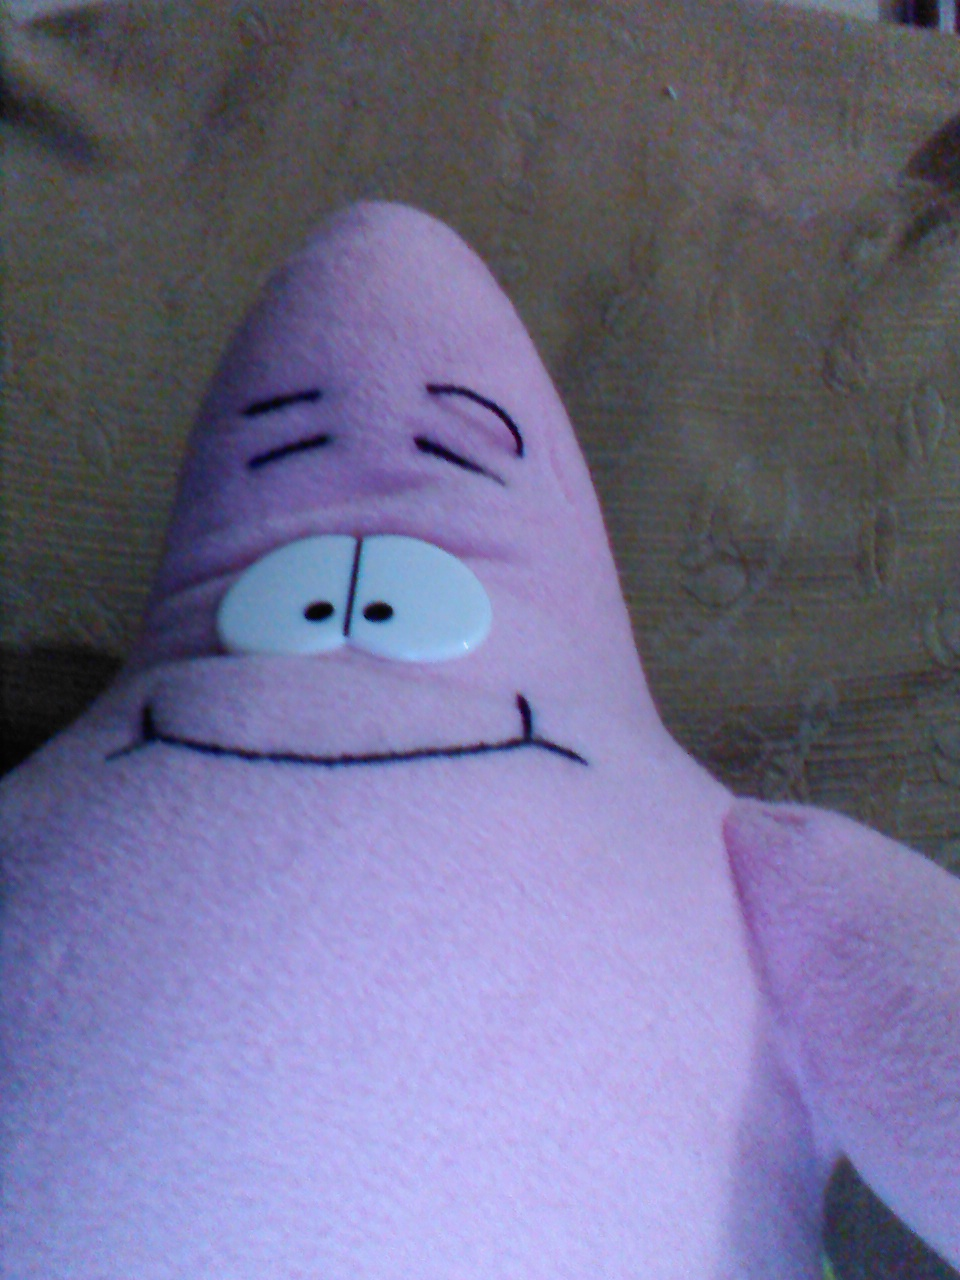
\includegraphics[width=0.27\textwidth]{imagenes_usuario/foto.jpg}
		\endgroup
	\end{center}


El usuario tiene la opción de cambiar la foto de los recuadros cuantas veces desee.
La plantilla está lista para convertirse en una caricatura.
El usuario tendrá las opciones de agregar a su plantilla, íconos con textos divertidos  y con diseños propios de los autores de Comic It!
\newline
\newline

\begingroup
		\large{
			\textbf{
				Iconos...
				\newline
				\newline
			}
		}
	\endgroup
Al escoger la opción de Symbols en los Tabs superiores, se abrirá una ventana que muestre la variedad de símbolos que el usuario puede escoger según lo que más se ajuste al tipo de caricatura que esté creando. Una vez escogido el símbolo, éste aparecerá en la plantilla que contiene las fotos anteriormente escogidas.
	\begin{center}
		\begingroup
			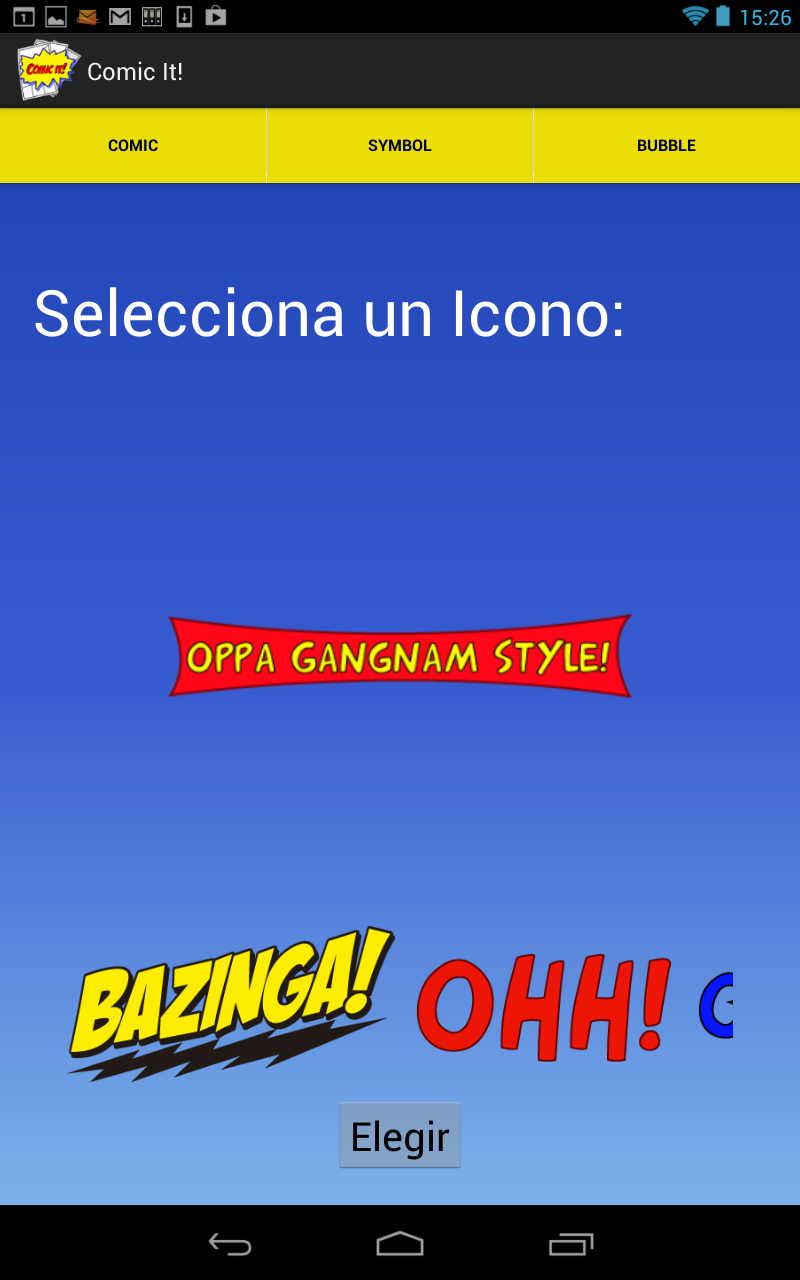
\includegraphics[width=0.30\textwidth]{imagenes_usuario/iconos.png}
		\endgroup
	\end{center}


\begingroup
		\large{
			\textbf{
				Burbujas...
				\newline
				\newline
			}
		}
	\endgroup
El usuario tendrá la opción de arrastrar el ícono escogido en cualquier espacio de la plantilla. Podrá repetir el proceso con el número de íconos que desee colocar en su caricatura.
Al escoger la opción de Burbujas en los Tabs superiores, se abrirá una ventana que muestre la variedad de colores de burbujas que el usuario puede escoger según lo que más se ajuste al tipo de caricatura que esté creando. Una vez escogido el color de la burbuja, el usuario podrá escribir el texto que desee que esté en el interior de dicha burbuja; al terminar este proceso, la burbuja editada (con su correspondiente texto y color) aparecerá en la plantilla que contiene las fotos anteriormente escogidas.

	\begin{center}
		\begingroup
			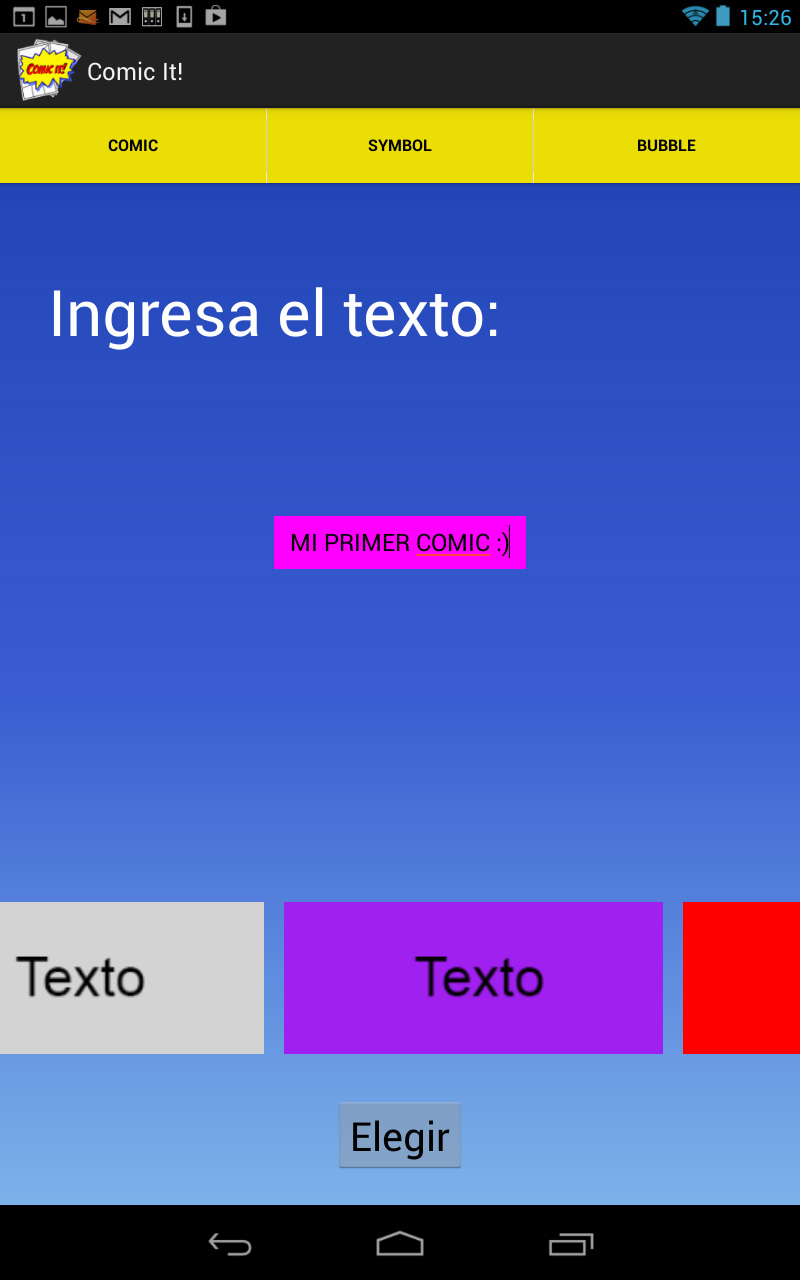
\includegraphics[width=0.27\textwidth]{imagenes_usuario/texto.png}
		\endgroup
	\end{center}

%--------------------------------------------------------------------------------------------------------------------


\begingroup
		\large{
			\textbf{
				Colocando imágenes...
				\newline
				\newline
			}
		}
	\endgroup
El usuario tendrá la opción de arrastrar la burbuja escogida en cualquier espacio de la plantilla. Podrá repetir el proceso con el número de burbujas que desee colocar en su caricatura.
\newline


	\begin{center}
		\begingroup
			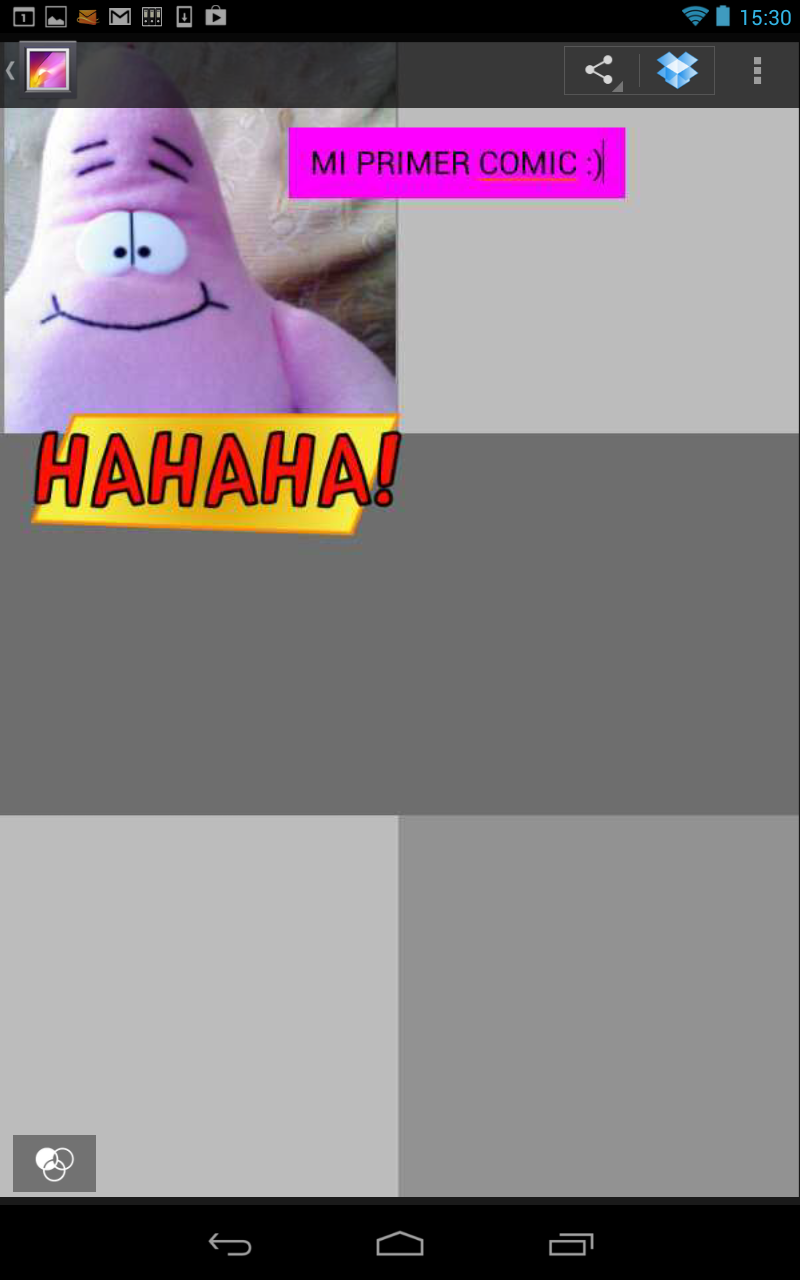
\includegraphics[width=0.27\textwidth]{imagenes_usuario/comic.png}
		\endgroup
	\end{center}

%--------------------------------------------------------------------------------------------------------------------


\begingroup
		\large{
			\textbf{
				Compartiendo nuestra caricatura
				\newline
				\newline
			}
		}
	\endgroup
Presionar el botón guardar para que la caricatura se guarde en la memoria del celular.
Hoy en día las redes sociales son muy utilizadas en cualquier actividad que realicemos. ¿Por qué no compartir nuestra experiencia con amigos o familiares?
Por esto Comic It! permite compartir tu experiencia en Facebook.
\newline

	\begin{center}
		\begingroup
			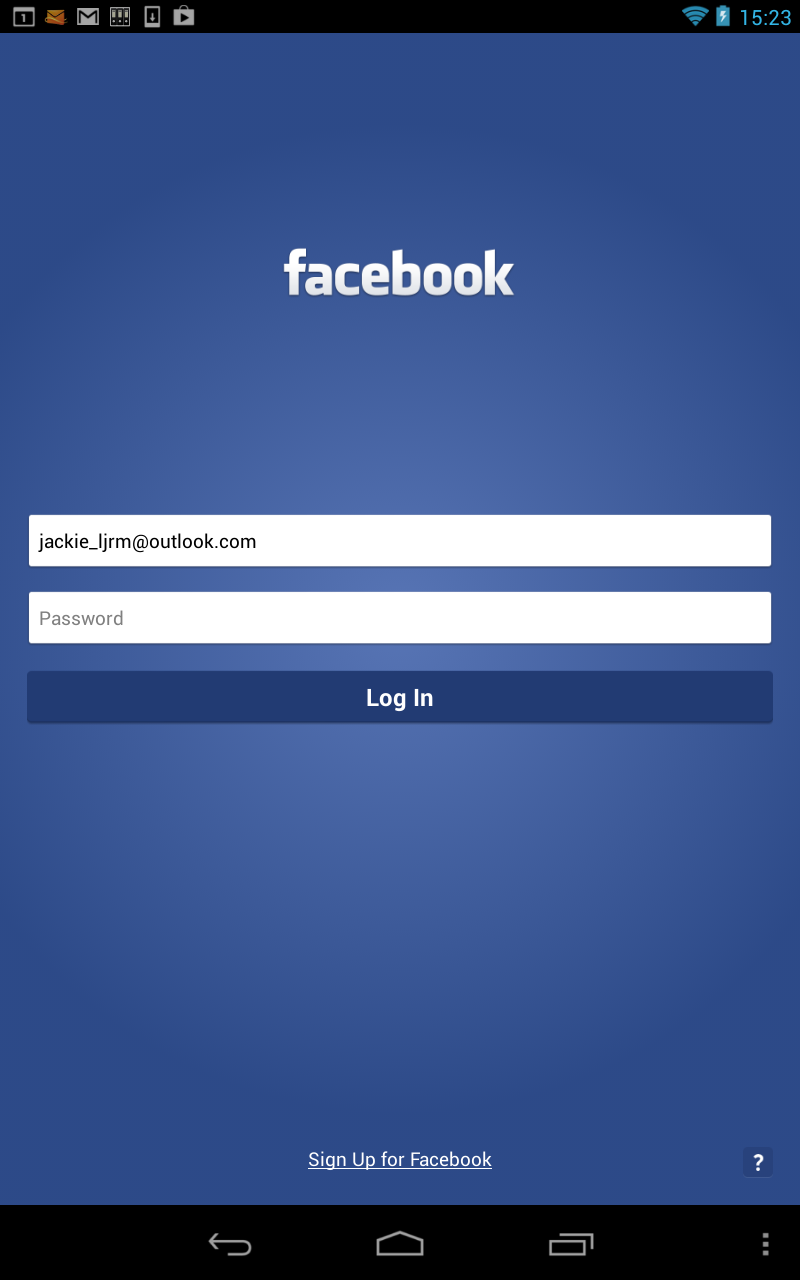
\includegraphics[width=0.27\textwidth]{imagenes_usuario/face.png}

		\endgroup
	\end{center}


 \ref{capitulodos}



%---------------------------------------------------------------------------------------------------------------------------------
%--------------------------------------------------------------ENTREGA TU TAREA------------------------------------------
%---------------------------------------------------------------------------------------------------------------------------------

\chapter{Proyecto Python\label{capitulotres}}
\begin{center}
		\Huge{\textbf{\\Entrega Tu Tarea!	\vspace{1em}}}
\end{center}	


	\begin{center}
		\begingroup
			
\includegraphics[width=0.35\textwidth]{imagenes_usuario/tarea.jpg}
		\endgroup
	\end{center}



	\begingroup
		\large{
			\textbf{
				Objetivo General
				\newline
				\newline
			}
		}
	\endgroup
	Definir y dar a conocer las funcionalidades y los requerimientos que tendrá el proyecto para la materia Lenguajes de 				
	Programación de la Escuela Superior Politécnica del Litoral. 

	\vspace{4em}
	\begingroup
		\large{
			\textbf{
				Objetivos Específicos
				\newline
			}
		}
	\endgroup
		\begin{enumerate}[(a)]%for small alpha-characters within brackets.
		\item Conocer las funcionalidades de la nueva aplicación en Python: Entrega Tu Tarea!.
		\item Describir cada una de las funcionalidades que tendrá la aplicación.
		\item Especificar quiénes serán los usuarios finales de la aplicación.
		\item Presentar ciertas características que tendrá la aplicación final.

		\end{enumerate}

	\begingroup
		\large{
			\textbf{
				\newline
				\newline
				\newline
				\newline
				Descripción
				\newline
				\newline
			}
		}
	\endgroup

	%
	%Descripcion
	%
``Entrega tu Tarea! Es un divertido juego, con orientación educativa, puesto que de una forma entretenida, los niños podrán ejercitar su mente, sus habilidades matemáticas a través de un sano juego.
\newline
\newline
``Entrega tu Tarea tendrá como usuarios niños de jardin (4-5 años)  y de escuela (7-12 años). El objetivo es que el usuario vaya estructurando una tarea que consta de 3 partes: habilidad con la memoria, habilidades matemáticas, y habilidades visuales; otro objetivo es que el usuario pueda seguir correctamente las instrucciones que se le dan por medio de un audio.
\newline
\newline
Con una serie de audios e imágenes el usuario manejará facilmente este juego, y empezará a relacionar tareas diarias escolares con algo entretenido y práctico
\newline
\newline
Este juego está desarrollado en Python utilizando la librería Pygame, y como herramientas adicionales se utilizó Adobe Photoshop para la creación de imágenes y Audacity para la creación de audios.
	\newline
	\newline
	\newline
	\begingroup
		\large{
			\textbf{
				Funcionalidades
				\newline
				\newline
			}
		}
	\endgroup
	%
\newline
Entrega tu Tarea cuenta con muchas funcionalidades. Es un juego en el que con el paso de los niveles el usuario obtendrá cada vez mas habilidades.
\newline
\newline
La primera funcionalidad es la parte llamada "Memoriza", en esta parte el usuario tendrá que escuchar un audio con una secuencia de letras y números y despues ingresar correctamente dicha secuencia por teclado.
\newline
\newline
La segunda funcionalidad es la "Tarea matemática"  que consta de un ejercicio matemático conforme al nivel estudiantil y años que tiene el usuario, datos que se piden en el transcurso del juego.	
\newline
\newline	
Finalmente si el usuario ha respondido correctamente las tareas anteriores, tendrá que pasar por un divertido juego en el que tendrá que superar una serie de obtaculos para poder entregar su tarea exitosamente.
\newline
\newline
En el transcurso del juego, el usuario tendrá que seguir las instrucciones proporcionadas en audio.
\newline
\newline
El juego está hecho de forma que el usuario ingrese su nivel educativo(Jardín o escuela) y su edad; con estos datos, el programa escogerá que tipo de ejercicios matemáticos son los adecuados para la tarea.

\newpage

%--------------------------------------------------------------------------------------------------------------------
\begin{center}
	\begingroup
		
		\Huge{\textbf{\\Manual de Usuario	\vspace{1em}}}

	\endgroup
\end{center}
Inicio del juego. Escoja la opción que desee. Si desea jugar directamente, escoja por medio de las direccionales qué nivel educativo tiene y presione enter. Si desea conocer acerca de los creadores del programa, diríjase a la opción Creadores y presione enter


	\begin{center}
		\begingroup
			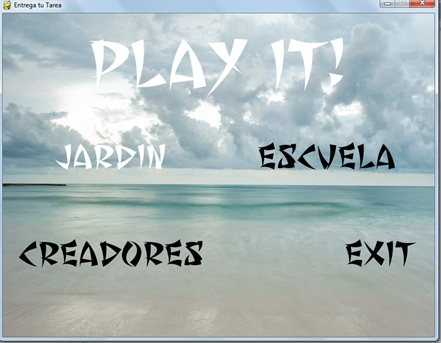
\includegraphics[width=0.6\textwidth]{imagenes_usuario/inicio.jpg}
		\endgroup
	\end{center}


%--------------------------------------------------------------------------------------------------------------------

Al escoger el nivel jardin o el nivel escuela, escuchará un audio con instrucciones. Esta es la tarea de "Memoria", memorice la secuencia e ingresela por teclado, al terminar de ingresar dicha secuencia presione la tecla F5.

	\begin{center}
		\begingroup
			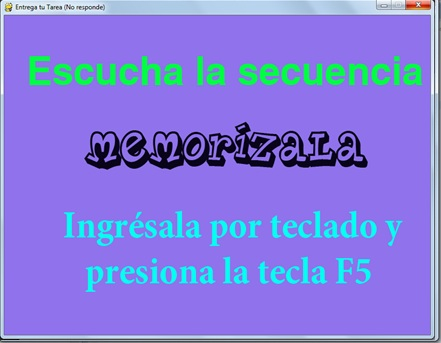
\includegraphics[width=0.6\textwidth]{imagenes_usuario/memoriza}
		\endgroup
	\end{center}

%--------------------------------------------------------------------------------------------------------------------

Inmediatamente saldrá un audio junto con una imagen que pedirán su edad, ingrésela por medio del teclado y cuando haya terminado presione la tecla F3

	\begin{center}
		\begingroup
			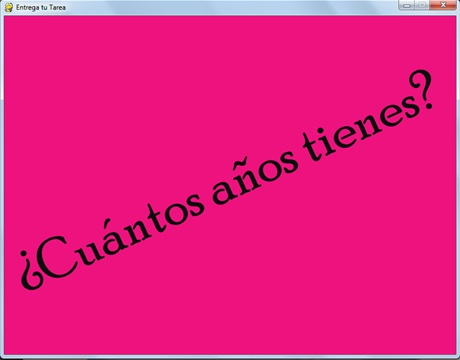
\includegraphics[width=0.6\textwidth]{imagenes_usuario/anios.jpg}
		\endgroup
	\end{center}


%--------------------------------------------------------------------------------------------------------------------

Después de haber ingresado su edad, pasará a la "Tarea Matemática", escuchará una serie de instrucciones y aparecerá una imagen con un ejercicio de matemáticas conforme al nivel educativo que ingresó al comienzo (Jardín o escuela) y de acuerdo a la edad que proporcionó anteriormente.
Resuelve el ejercicio, no hay límite de tiempo. Si se está seguro de la respuesta ingrésela por medio del teclado y presione la tecla F4.
Si la respuesta es incorrecta, escuchará un audio que le dirá que tiene una segunda oportunidad. El límite de equivocaciones es 3, si se equivoca mas de 3 veces, perderá.

	\begin{center}
		\begingroup
			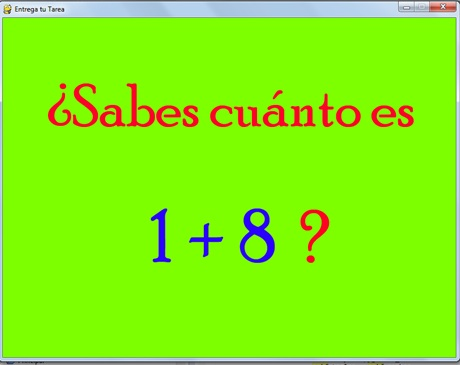
\includegraphics[width=0.6\textwidth]{imagenes_usuario/ejercicio.jpg}
		\endgroup
	\end{center}


%--------------------------------------------------------------------------------------------------------------------

Si se contestó correctamente, se pasará al juego, en el que se tendrá que pasar una serie de obstáculos para poder entregar su tarea exitosamente.
Escuchará las instrucciones respectivas del juego.
Muévase con las teclas direccionales (derecha: mover derecha, izquierda: mover izquierda, arriba: saltar) y dispare a las caritas felices con la tecla 1.

	\begin{center}
		\begingroup
			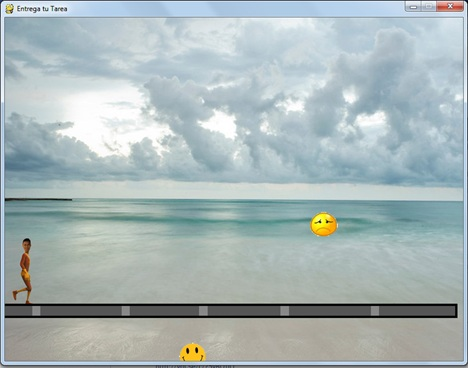
\includegraphics[width=0.6\textwidth]{imagenes_usuario/juego1.jpg}
		\endgroup
	\end{center}

%--------------------------------------------------------------------------------------------------------------------

Si se realizaron todas las tareas completamente, el usuario habrá ganado y entregado su tarea con exito!

	\begingroup
		\large{
			\textbf{
				\newline
				\newline
				\newline
				Experiencias con Python y Pygame
				\newline
				\newline
			}
		}
	\endgroup
	%

Cuando empezamos a estudiar Python, al iniciar este proyecto, nos encantó este lenguaje, nos pareció sencillo y totalmente completo; lo que nos pareció más interesante es la facilidad en la sintaxis del lenguaje, no es muy estricto como los otros lenguajes que dan mil errores por la falta de un punto y coma; sin embargo python se guía de manera excelente solo con identación; aunque nunca le habíamos puesto tanto interés en la identación, ahora lo hacemos  y lo haremos en cualquier lenguajes aunque no se trate de python.
\newline
\newline
Con respecto a Pygame, nos parecieron increíbles todas las funcionalidades que éste ofrece.
Al utilizar un ciclo while los juegos realizados en pygame, el manejar la actualizacion de los diferentes estados del juego (interfaz grafica) resultó un poco tedioso realizar el cambio de pantallas de nuestra aplicación.
\newline
\newline
El manejo de Sprites y GroupSprites disponibles en pygame nos resulto "mágico" debido a que esta clases nos provee mucha funcionalidades muy interesantes como por ejemplo para dibujar un objeto en pantalla ke herede de Sprite tan solo es necesario utilizar "el rectángulo e imagen del objeto" y el uso GroupSprites son un conjunto de Sprites y para dibujarlos hace uso de cada uno de los rectangulos e imagens de los Sprites que se encuentran en el grupo...
por esto darla apariencia de movimiento e interaccion del objeto tan solo fue necesario actualizar su posicion en pantalla (puntos x,y) y con estos actualizar el rectangulo del objeto.
\newline
\newline
Al comienzo del proyecto parecía un poco exagerado esto de hacer un “Video Juego” pero en el transcurso del proyecto esto se fue convirtiendo en una tarea más fácil y entretenida. Nos gustó mucho programar un Video Juego, espero mejorarlo con el tiempo.
En resumen fue una linda experiencia trabajar en este proyecto.
\newline
\newline
Como recomendación diría que el modularizar el proyecto es una muy buena practica de programación, ya que se obtiene un código mas organizado y facilidad para acceder a las funcionalidades que deseamos que tenga nuestro proyecto.
\newline\newline
\newline\newline
\newline\newline
\newline\newline
\newline\newline
\newline\newline
\newline\newline
\newline\newline
\newline\newline
\newline\newline
\newline\newline
\newline\newline
\newline\newline
\newline\newline
\newline



 \ref{capitulotres}




%---------------------------------------------------------------------------------------------------------------------------------
%--------------------------------------------------------------LA AVENTURA DE SAKURA------------------------------------------
%---------------------------------------------------------------------------------------------------------------------------------
\newpage
\chapter{Proyecto Python\label{capitulocuatro}}
\begin{center}
		\Huge{\textbf{\\La Aventura de Sakura	\vspace{1em}}}
\end{center}	

	\begin{center}
		\begingroup
			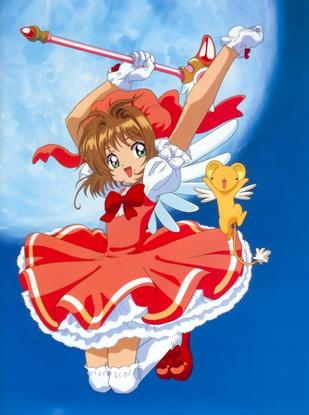
\includegraphics[width=0.6\textwidth]{imagenes_usuario/sakura.jpg}
		\endgroup
	\end{center}

	\begingroup
		\large{
			\textbf{
				Objetivo General
				\newline
				\newline
			}
		}
	\endgroup
	Definir y dar a conocer las funcionalidades y los requerimientos que tendrá el proyecto para la materia Lenguajes de 				
	Programación de la Escuela Superior Politécnica del Litoral. 

	\vspace{4em}
	\begingroup
		\large{
			\textbf{
				Objetivos Específicos
				\newline
			}
		}
	\endgroup
		\begin{enumerate}[(a)]%for small alpha-characters within brackets.
		\item Conocer las funcionalidades de la nueva aplicación en Python: Entrega Tu Tarea!.
		\item Describir cada una de las funcionalidades que tendrá la aplicación.
		\item Especificar quiénes serán los usuarios finales de la aplicación.
		\item Presentar ciertas características que tendrá la aplicación final.

		\end{enumerate}

	\begingroup
		\large{
			\textbf{
				\newline
				\newline
				\newline
				\newline
				Descripción
				\newline
				\newline
			}
		}
	\endgroup

	%
	%Descripcion
	%

``La Aventura de Sakura es un juego a base de audios, sin interfaz alguna, se logra una interacción agradable con el usuario, se logra crear un ambiente divertido sin necesidad de interacciones en la pantalla.
\newline
\newline
``Entrega tu Tarea tendrá como usuarios personas que carezcan de visión; ésto es lo que hace que éste juego sea muy útil para la sociedad. "La Aventura de Sakura" busca que el usuario interactue con el juego a través de comando simples que ingresará por teclado según las instrucciones que escuche en cada audio.
\newline
\newline
Esun juego sin mucha dificultad, sin embargo el usuario tendría que conocer las posiciones de las teclas para poder presionar las opciones que desee; de no ser así se recomienda ayuda externa.
\newline
\newline
Este juego está desarrollado en Python utilizando la librería Pygame para generar los audios y la interaccion por medio de teclado; los audios fueron grabados en el programa Audacity con formato .wav


\newpage
\begin{center}
	\begingroup
		
		\Huge{\textbf{\\Manual de Usuario	\vspace{1em}}}

	\endgroup

\end{center}
%-------------------------------------historaaa inicio---------------------------------------------------------

Sakura es una niña muy extrovertida, siempre risueña, y buena estudiante.
Un día Sakura queda sola en su casa, su padre y su hermano se habían ido a trabajar; de pronto escucha un sonido extraño en el sótano de su casa. Sakura se asustó mucho, tenía que tomar una decisión:
\newline
\newline
1.	Llamar a la policía
\newline
\newline
2.	Ir a averiguar que sucedía ella misma
\newline
\newline

Si escoges la opción 1:
\newline
\newline
Sakura llama a la policía. La policía llega en 45 minutos como es costumbre en Ecuador, y al entrar en su casa se dan cuenta que no había nada en el sótano. Sakura se ganó una multa porque se consideró que estaba jugando con el tiempo de la policía.
\newline
\newline
Si escoges la opción 2:
\newline
\newline
Sakura cogió su bastón de porrista y se dirigió en silencio al sótano, abrió lentamente la puerta y estaba muy oscuro
\newline
\newline
Sakura aún no está segura si bajar al sótano.
\newline
\newline

1.	Sakura se retracta y llama a la policía
\newline
\newline
2.	Sakura se llena se valor y va a averiguar que sucede
\newline
Si escoges la opción 1:
\newline
\newline
Sakura llama a la policía. La policía llega en 45 minutos como es costumbre en Ecuador, y al entrar en su casa se dan cuenta que no había nada en el sótano. Sakura se ganó una multa porque se consideró que estaba jugando con el tiempo de la policía.
\newline
\newline

Si escoges la opción 2:
\newline
\newline

Sakura baja lentamente las escaleras, recorre el sótano y se da cuenta que no había nadie. Pero de pronto se dio cuenta que misteriosamente uno de los libros que se encontraban en el sótano brillaba intensamente; que hará Sakura?
\newline
\newline
1.	Sakura se retracta y llama a la policía
\newline
\newline
2.	Sakura abre el libro y averigua de que se trata este misterio
\newline
\newline
Si escoges la opción 1:
Sakura llama a la policía. La policía llega en 45 minutos como es costumbre en Ecuador, y al entrar en su casa se dan cuenta que no había nada en el sótano. Sakura se ganó una multa porque se consideró que estaba jugando con el tiempo de la policía.
\newline
\newline
Si escoges la opción 2:
\newline
\newline
Sakura abre el libro y una fuerte ráfaga de viento sale fuertemente desde el libro. Una serie de cartas salen volando y atraviesan el techo y se dispersen por todo el cielo, sin embargo sakura pudo tomar 2 en su mano. Las cartas viento y agua. De repente un simpático personaje entra en escena y le dice a Sakura.  Yoo soy el guardián de este libro, mi nombre es Kerberos quien eres tuu?
Sakura le responde con una pregunta y le dice: Tú eras el que hacías ruido con tus ronquidos?
Kerberos le responde avergonzado: yo no ronco aunque he estado dormido hace 400 años. Mi deber es proteger las cartas que ves aquí, señalando el libro, pero no había ya ninguna carta, todas habían volado ya.
Sakura le cuenta a kero que las cartas salieron volando.
Kerberos pega un gritoo al cielo y le dice a Sakura: Ohhh nooo!! Ahora es tu misión recolectar nuevamente las llamadas cartas clow, ya que si estas están sueltas pueden destruir el mundo.
\newline
\newline
Sakura se queda helada, debe tomar una decisión:
\newline
\newline
1.	Rechaza la misión y deja que el mundo se destruya poco a poco.
\newline
2.	Acepta la misión y recolecta todas las cartas, lo cual es una misión muy peligrosa.
\newline
Si escoges la opción 1:
\newline
\newline
El mundo entra en caos y nadie puede hacer nada, el fin del mundo ha llegado por la falta de valentía de Sakura. Fin
\newline
\newline
Si escoges la opción 2:
\newline
\newline
La siguiente noche cerca de la casa de sakura hubo un incendio que ni siquiera los bomberos podían apagar. Kerberos que se encontraba junto a sakura, sintió la presencia de una carta Clow, él estaba seguro que ese incendio tuvo que ser ocasionado por algún poder extraño ya que no se trataba de un incendio normal.
Kerberos le dice a Sakura que su misión inicia en ese momento. Sakura contaba con 2 cartas clown: Agua, viento y vuelo.
Tenía que valerse de alguna de estas cartas para poder vencer al terrible Fuego.
Primero tenía que llegar al lugar del incendio. Como llegaría?
\newline
\newline
1.	Sakura llega al lugar con los patines con los que siempre se moviliza al colegio aunque  quizás cuando llegue ya no se pueda hacer nada.
\newline
\newline
2.	Sakura le tiene pánico a las alturas. Pero podía utilizar la carta del vuelo para llegar hasta allá.
\newline
\newline
Si escoges la opción 1:
\newline
\newline
Cuando llega sakura el fuego se extendió demasiado, muchas personas han muerto, y ya no se puede hacer nada, Sakura fracasó en su misión. Y las cartas se apoderaron del mundo entero. Fin
\newline
\newline
Si escoges la opción 2:
\newline
\newline
1.	Sakura utiliza la carta vuelo y llega rápidamente al incendio. Debe de tomar una decisión para poder extinguir el fuego:
	Sakura utiliza la carta agua.
\newline
2.	Sakura utiliza la carta viento
\newline
\newline
Si escoges la opción 1:
\newline
\newline
1.	Sakura utiliza la carta Agua y logra vencer el fuego. Sakura cumplió exitosamente su misión y tiene una carta más que podrá utilizar en sus futuras misiones.
\newline
\newline
Si escoges la opción 2:
\newline
\newline
2.	Sakura utiliza el viento, y este hace que el fuego se haga aún más grande; el fuego se extendió demasiado, muchas personas han muerto, y ya no se puede hacer nada, Sakura fracasó en su misión. Y las cartas se apoderaron del mundo entero. Fin

%-------------------------------------historaaa fin---------------------------------------------------------

	\begingroup
		\large{
			\textbf{
				\newline
				\newline
				\newline
				Experiencias con Python y Pygame
				\newline
				\newline
			}
		}
	\endgroup
	%

Al haber realizado el proyecto del capitulo 4 antes que éste, me resultó mucho mas fácil la elaboración de éste proyecto.
Python combinado con pygame son herramientas muy útiles y sencillas; al ser éste proyecto con solo audios, simplemente debiamos usar funcionalidades de pygame y manejar los eventos correctamente.
Lo mas tedioso de este proyecto fue la grabación de los audios.

Como recomendación, es bueno comprimir los audios, ya que si se los mantiene con su formato normal, el proyecto llega a pesar mucho, mas aún si se trata de un proyecto mas extenso.



 \ref{capitulocuatro}



%---------------------------------------------------------------------------------------------------------------------------------
%--------------------------------------------------------------MASTERMIND---------------------------------------------------
%---------------------------------------------------------------------------------------------------------------------------------

\chapter{Proyecto Haskell\label{capitulocinco}}
\begin{center}
		\Huge{\textbf{\\MasterMind	\vspace{1em}}}
\end{center}	

	\begin{center}
		\begingroup

			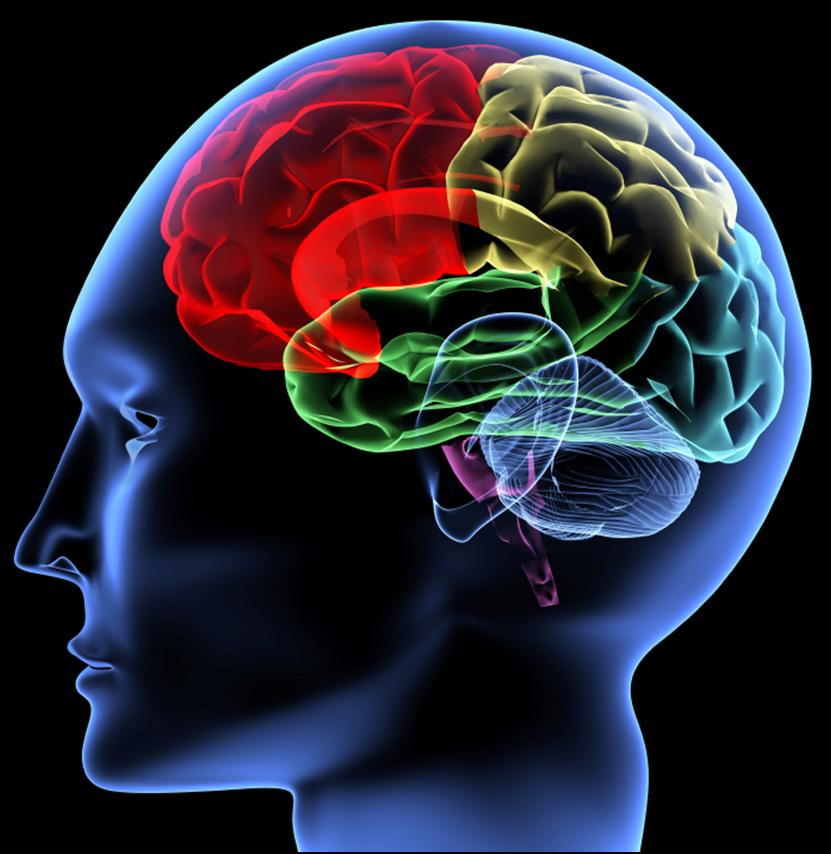
\includegraphics[width=0.4\textwidth]{imagenes_usuario/mastermind.jpg}
		\endgroup
	\end{center}

	\begingroup
		\large{
			\textbf{
				Objetivo General
				\newline
				\newline
			}
		}
	\endgroup
	Definir y dar a conocer las funcionalidades y los requerimientos que tendrá el proyecto para la materia Lenguajes de 				
	Programación de la Escuela Superior Politécnica del Litoral. 

	\vspace{4em}
	\begingroup
		\large{
			\textbf{
				Objetivos Específicos
				\newline
			}
		}
	\endgroup
		\begin{enumerate}[(a)]%for small alpha-characters within brackets.
		\item Conocer las funcionalidades de la nueva aplicación en Haskell: MasterMind.
		\item Describir cada una de las funcionalidades que tendrá la aplicación.
		\item Especificar quiénes serán los usuarios finales de la aplicación.
		\item Presentar ciertas características que tendrá la aplicación final.

		\end{enumerate}

	\begingroup
		\large{
			\textbf{\newline
				\newline
				Descripción
				\newline
				\newline
			}
		}
	\endgroup

	%
	%Descripcion
	%

``Mastermind (Español "Mente maestra") es un juego de mesa, de ingenio y reflexión, para dos jugadores.
Se juega en un tablero con fichas blancas y negras pequeñas y de otros colores, de un tamaño algo superior. Uno de los jugadores escoge un número de fichas de colores, 4 en el juego original, y pone un código secreto oculto del otro jugador. Éste, tomando fichas de colores del mismo conjunto, aventura una posibilidad contestada con negras (fichas de color bien colocadas) o blancas (fichas de color con el color correcto, pero mal colocadas).
Termina al averiguarse la combinación (es decir, se consigue una combinación con cuatro negras), o bien se agota el tablero (depende del tamaño, aunque generalmente son 15 combinaciones).

	\begingroup
		\large{
			\textbf{\newline
				\newline
				Experiencias con Haskell
				\newline
				\newline
			}
		}
	\endgroup

El proyecto de Haskell a mi parecer fue el proyecto en el que mas se tuvo que estudiar del libro y tutoriales ya que al manejarse con un paradigma diferente, al programar debemos tener otras prácticas, modalidades, es decir, la mayor parte de practicas de programación que utilizaba frecuentemente, se utilizaron muy poco en este proyecto.
La recursividad es una de las propiedades mas destacadas que me gustaria mencionar; es muy bueno el utilizar recursión para hacer nuestro codigo mas eficiente y corto, mientras menos lineas mejor.



 \ref{capitulocinco}





\end{document}